\subsection{Подготовка клиентов}

Для того, чтобы подготовить к работе терминал, нужно установить ОС, RDP-клиент, и 
настроить автоматическое подключение к серверу.

С официального сайта \cite{ref:raspbian} необходимо скачать iso-образ Raspbian, версии
Lite без рабочего стола. Для установки ОС на microSD карту используется Etcher
\cite{ref:etcher}. 

\begin{figure}[h]
    \center
    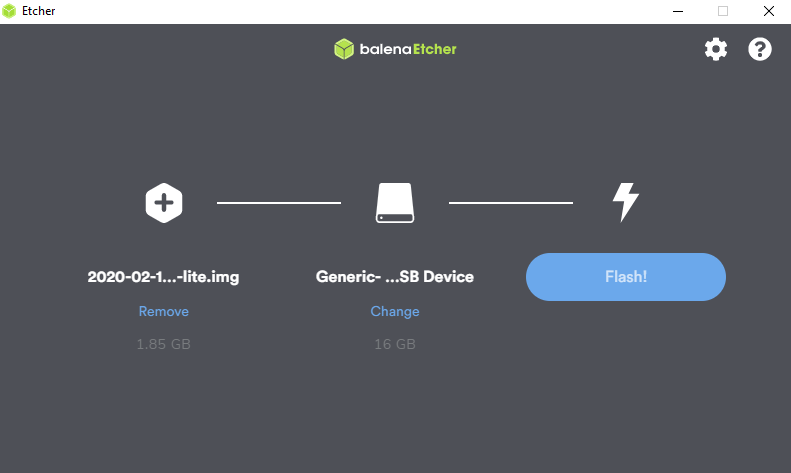
\includegraphics[height=10cm]{rpi-etcher}
    \caption{Запись iso на SD-карту с помощью Etcher}
    \label{pic:rpi-etcher}
\end{figure}

